\chapter{System Theory}
\label{chap:sysdes}
To understand the problem and the procedure to examine the fatigue of dynamic power cables in wind farms, a fundamental understanding of the system is required. This chapter covers theory for wind turbines in general and offshore wind turbines as well as subsea power cables. The chapter also includes historical background, some principal mathematical background, and other relevant theory. 
\section{Wind Turbines}
A wind turbine can convert kinetic energy into mechanical energy, and then to electric energy. This conversion is done by extracting the kinetic energy of an air stream by the use of a rotating, disk-shaped wind energy converter, \cite{Hau2013}.

\subsection{Historical Background of Wind Turbines}
According to \cite{Wagner2013}, man has utilized energy from the wind for thousands of years. In the earliest years, wind energy was mainly used as propulsion for sailing vessels. There are accounts of windmills in Persia as early as 914 AD, and in Europe from around 1200 BC. The first windmills were used for pumping of water and grinding of cereal. Between 1700-1800 there was a major spurge in windmill technology, and new designs with higher efficiency emerged. \cite{Lynn2011} states that before the industrial revolution, windmills were an important source of mechanical energy in Europe. Denmark, England, Germany, and the Netherlands were among the countries with the most development. Windmill technology experienced even more growth in the twentieth century, and in early 1900 multi-blade wind farms were developed in the US. At this time, the wind energy was used to convert kinetic energy into mechanical energy, \cite{Hau2013}. According to \cite{Lynn2011}, as the industrial revolution emerged, the advancement of windmills declined. Steam engines and combustion motors could provide power at any time, efficiently and independent of weather conditions. Electrical motors could be used to grind grains and pump water more effectively than ever. By the mid-1900s it was rare to see a traditional windmill still in service. \newline 
\newline
As electricity technology evolved, the notion of utilizing windmills to generate electrical power arose. One of the most remarkable people behind this approach was Charles Brush. As early as 1888 he developed "A multi-blade rotor 17 m in diameter, [...]a 12 kW dynamo charged a battery bank that fed various motors and hundreds of incandescent lights in his home over the next 15 years", \cite{Lynn2011}. This was the first \textit{wind turbine}. In the following years, there was enormous progress in the design and performance of wind turbines. \cite{Hau2013} describes the emergence of the modern wind turbine with the unit created by Ulrich Hütter. He published papers on the theory of wind energy in 1942 and is said to be one of the pioneers of modern wind energy technology. Hütter built wind turbines with fewer blades, that were profoundly aerodynamically refined, and designed for a greater rotation speed than was seen previously. According to \cite{Wagner2013}, this was particularly beneficial, as only a small generator was required to generate electricity. Figure \ref{fig:hutter} shows a windmill by Hütter, and as can be seen, it is quite similar to the windmills one usually encounters today. \newline
\newline

\begin{figure}[H]
\centering
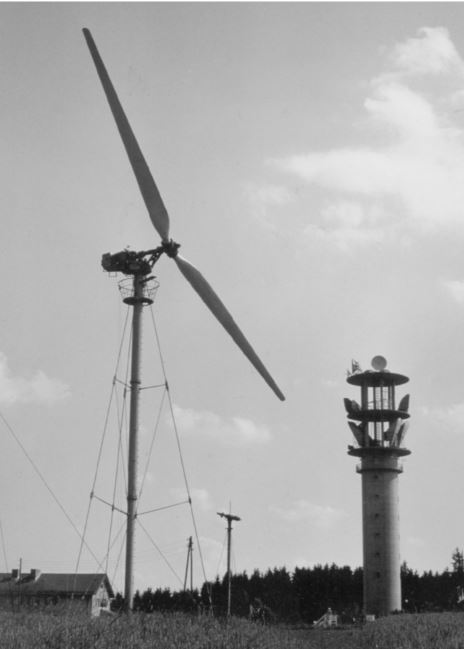
\includegraphics[scale=0.6]{figures/hutter}
\caption[$\; \:$Hûtter Wind Turbine Concept]{"Wind turbine by U. Hütter in Stötten in the Swabian Alb, Germany (rotor diameter 34 m, rated power 100 kW), 1958-1968", \cite{Hau2013} }
 \label{fig:hutter}
\end{figure}

\noindent \cite{Lynn2011} describes the 200kW wind turbine designed and built by the Dane Johannes Juul in 1957 as one of the most prominent concepts leading up to the modern wind turbine. It had stall control, and emergency aerodynamic tip breaks to avert damage in extreme weather. In 1975 it was refurbished by NASA to be used in their wind energy program. This turbine put Denmark on the map as one of the principal wind energy nations. 
\newline 
\newline
\noindent In spite of the dramatic increase in efficiency attained by the new technology, energy from wind turbines did not prove to be competitive compared to other sources of electricity in the 1960s to 1970s. It was not until the oil crisis in the seventies that several countries recognized that the world would eventually be dependent on other energy sources than fossil fuels sometime in the future, \cite{Wagner2013}.  President Jimmy Carter ensured the financing for several extensive wind projects, and by the early 1980s, the state of California had thousands of wind turbines with a combined power production of 1 GW. Nevertheless, this development stalled as President Reagan withdrew the financing of many projects, making Europe, and especially Denmark and Germany the leading nations in wind turbine technology. 
\cite{Lynn2011}

\subsection{Mathematical Background of Wind Turbines}
The concept of a wind turbine, independently of type, is to convert kinetic energy in the wind into mechanical energy, using a disk shape rotating wind energy converter. The mechanical energy is used to generate electrical energy.  According to \cite{Hau2013},  Albert Betz was the first to implement this principle to windmills, and developed theory where he applied elementary physics to wind converts. The theory contains simplifications such as assumed frictionless flow; however, it has demonstrated to be quite useful in the early stages of calculation for practical engineering. The following part of the section was originally developed by Albert Betz and later reproduced by \cite{Hau2013}.

\subsubsection{Basics of Albert Betz Momentum Theory:}
\noindent Kinetic energy:
\begin{equation}
    E=\frac{1}{2} m v^2 \qquad (Nm)
\end{equation}
 where for a wind converter, v is the velocity of an air flow of mass m. The volume flow, $\dot V$ is:
 
 \begin{equation}
    \dot V= v A \qquad (m^3/s)
\end{equation}
where A is the area. The mass flow $\dot m$ is expressed as:

 \begin{equation}
    \dot m = \rho_{air} v A \qquad (kg/s)
\end{equation}

\noindent where $\rho_{air}$ is the density of air. The amount of energy passing through the cross section per unit time:

 \begin{equation}
    P = \frac{1}{2}\rho_{air} v^3 A \qquad (W)
\end{equation}

\noindent  The kinetic energy in the airflow decreases with the extraction of mechanical energy. Reducing the velocity means widening the area of the cross-section. This is depicted in Figure \ref{fig:flow}. Here $V_1$ and  $A_1$ refers to the flow velocity and area before the extraction of energy, and $V_2$ and $A_2$ refers to the flow velocity and area after the extraction.

\begin{figure}[H]
\centering
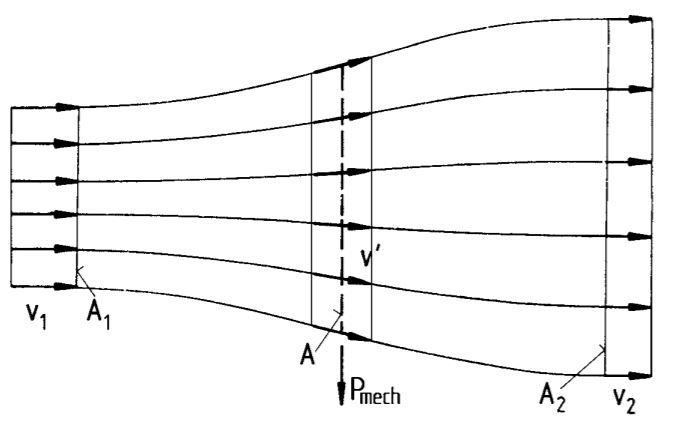
\includegraphics[scale=0.6]{figures/flow}
\caption[$\; \:$Changing flow conditions due to extracting of mechanical]{Changing flow conditions due to extracting of mechanical energy based on elementary momentum theory, \cite{Hau2013} }
 \label{fig:flow}
\end{figure}

\noindent The extraction of energy is due to the \textit{difference} in power before and after the extraction: 

\begin{equation}
    P = \frac{1}{2}\rho_{air} v^3_1 A_1 - \frac{1}{2}\rho_{air} v^3_2 A_2 =\frac{1}{2}\rho_{air}( v^3_1 A_1 - v^3_2 A_2) \qquad (W)
    \label{eq:air}
\end{equation}

\noindent From the Equation \ref{eq:air} it follows that the maximum energy extracted is obtained if $V_2=0$. Physically, however, this does not make sense as this implies that $V_1$ must become equal to zero, meaning no energy extraction at all. Through the conservation of momentum, Albert Betz developed a theory of the optimal relationship between the flow velocity before and after the extraction, $\frac{V_1}{V_2}$. $c_p$ was introduced to have a reference for the power output, where the power output, $P$  is compared the power of a free-flowing flow without extraction, $P_0$. 
  \begin{equation}
    C_P = \frac{P}{P_0}
\end{equation}

Figure \ref{fig:idealflow} show that the maximum power to be extracted is at $C_P$ close to 0.6, more precisely at: 
 \begin{equation}
    C_P = \frac{16}{27} = 0.593
\end{equation}

\noindent This is frequently called the Betz factor and expresses the maximum theoretical efficiency. 
\begin{figure}[H]
\centering
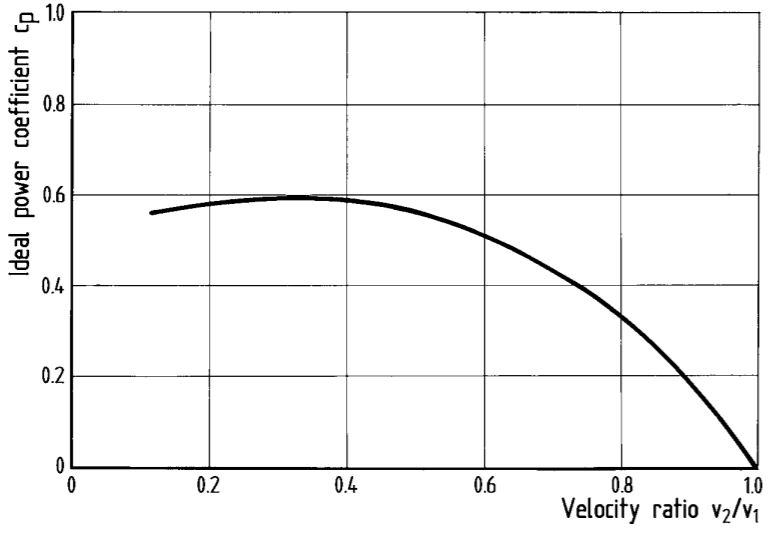
\includegraphics[scale=0.6]{figures/idealflow}
\caption[$\; \:$Power coefficient versus velocity ratio]{"Power coefficient versus velocity ratio" \cite{Hau2013} }
 \label{fig:idealflow}
\end{figure}

\subsubsection{Basics of Foil Theory}
One of the most fundamental components of the wind turbine are the blades. They are shaped as foils and are responsible for the transfer of the kinetic energy in the wind, to the mechanical energy of the rotor. \cite{MATHEW2012} states that in earlier days, the foils in wind turbines were adopted from airplane foils. Today,  there is a whole industry dedicated to the optimization and design of wind turbine foils. A basic illustration of the essential features of a standard airfoil is shown in Figure \ref{fig:foil}.  

\begin{figure}[H]
\centering
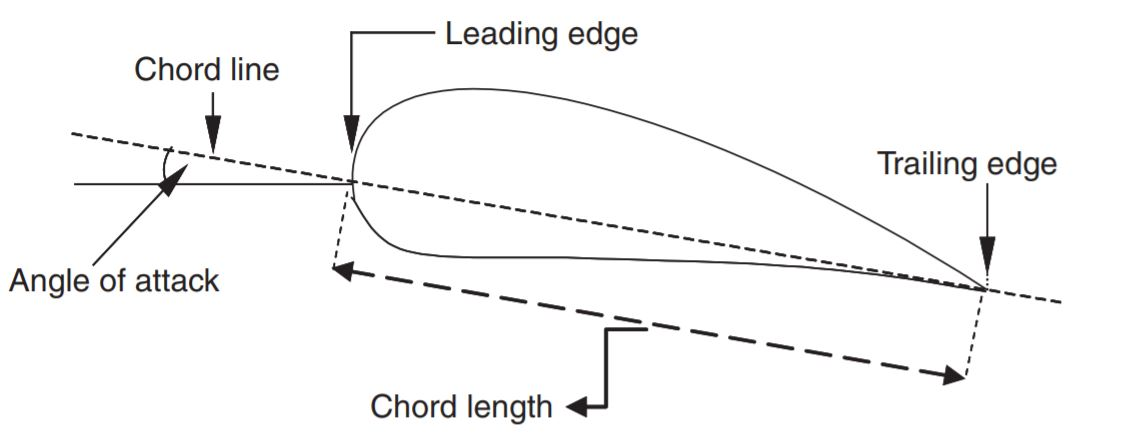
\includegraphics[scale=0.6]{figures/foil}
\caption[$\; \:$Basic features of a foil]{Basic features of a foil, \cite{MATHEW2012} }
 \label{fig:foil}
\end{figure}

\noindent If the foil is placed in a flow stream, the foil experiences a separation of streamlines above and below the foil. Due to the configuration of the foil shape, the streamlines above the foil have a longer way to travel than those below the foil. Because of this, the velocity of the flow on the upper side has to increase to meet the particles in the streamlines on the bottom of the foil at the trailing edge. According to Bernoulli's theorem, increased velocity has to be counterbalanced with a reduction in pressure. Decreased pressure creates a pressure difference between the upper and lower side of the foil resulting in a lift force directed upwards. At the same time, a drag force is also exerted on the foil. Their resultant is the net experienced force on the airfoil, as illustrated in Figure \ref{fig:liftdrag}. 

\begin{figure}[H]
\centering
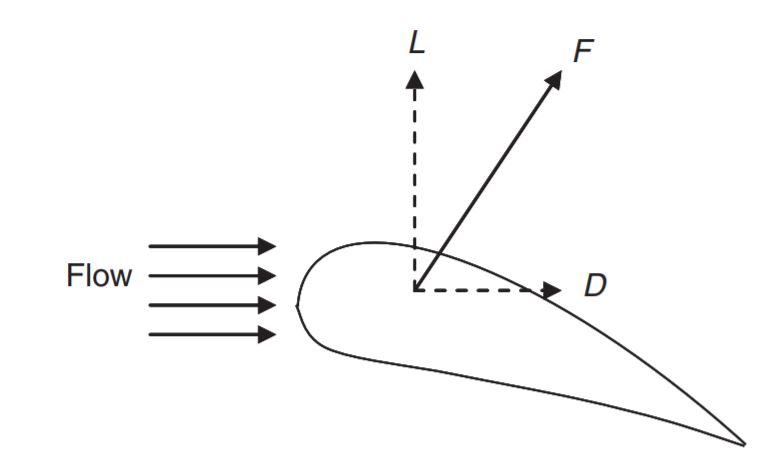
\includegraphics[scale=0.6]{figures/liftdrag}
\caption[$\; \:$Lift and drag on an airfoil]{Lift and drag on an airfoil, \cite{MATHEW2012} }
 \label{fig:liftdrag}
\end{figure}

 \noindent The lift and drag can be expressed as:

 \begin{equation}
    L = C_L\frac{1}{2}\rho_{air} v^2 A \qquad (N)
\end{equation}

\begin{equation}
    D = C_D\frac{1}{2}\rho_{air} v^2 A \qquad (N)
\end{equation}
Where $C_L$ and $C_D$ are lift and drag coefficients respectively.\newline 
\newline

\noindent The angle of attack influences the lift and drag forces (see Figure \ref{fig:foil}). In terms of airfoils used in wind turbines, the drag force is just a parasite component following the lift force, so it is a goal to maximize lift and minimize the drag so that the ratio $\frac{C_L}{C_D}$ reaches its maximum. For a wind turbine, the rotation of the foils creates a tangential velocity. The velocity experienced by a point is the resultant of the velocity and the tangential velocity. The drag force is parallel with the resulting velocity, and the lift is always perpendicular to the drag. 

\section{Offshore Wind Turbines}
The theory in the following paragraph is taken from \cite{Kapsali2012}.\\\\ In later years, there has been a significant increase in wind power installations. Renewable energy is on high demand, and wind energy is considered a cost-effective way of providing it. As restrictions on wind installations increase in terms of noise and visibility, development is being withheld. This has made a new market emerge: Offshore Wind Energy. Offshore wind energy implies electrical energy generated by wind installation placed offshore.  There are several advantages of this: wind speeds tend to increase with distance from shore, giving offshore wind energy an even greater potential than on-land wind energy. Also, the noise and visibility of the wind turbines are no longer a problem as long as the installation is placed far enough from shore, and the environmental impact is minimal. However, there are several challenges as well. The wind industry is a relatively new industry, and the ocean conditions such as weather, waves, currents, corrosion, and more, pose several challenges and demands multidisciplinary cooperation for development of plausible designs. New approaches are needed in terms of turbine, structure, installation, and maintenance, and the cost of offshore wind energy is considered higher than on land. Offshore wind energy generally follows a simple rule: The further from shore an installation is placed, the greater energy potential in terms of wind speed, but this also implies deeper waters and increased development and operation costs. A lot of the experience gained from the oil and gas industry is valuable in the advancement of offshore wind energy. 

\subsection{Historical Background for Offshore Wind Turbines}
\cite{NG2016} states that the first offshore wind farm was developed in Denmark in the 1990s. According to \cite{Lynn2011}, this wind farm consisted of 11 turbines providing 5 MW combined.  By using the already existing knowledge and technology both from the onshore windmill industry and the offshore oil and gas industry, offshore wind turbines have experienced rapid growth in the middle of the 2000s, with doubling of capacity every 2-4 years, \cite{NG2016}. Figure \ref{fig:development} shows the increase in offshore wind installations. \cite{Lynn2011} States that "It is reasonable that Europe will generate tens of gigawatts of offshore electricity by 2020".


\begin{figure}[H]
\centering
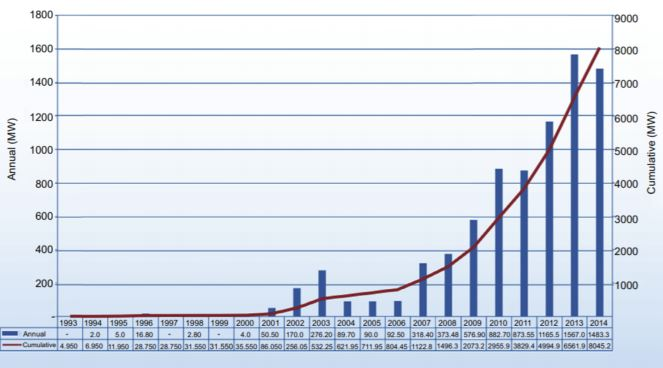
\includegraphics[scale=1.1]{figures/development}
\caption[$\; \:$Annual and cumulative offshore wind installations from 1993-2014]{Annual and cumulative offshore wind installations from 1993-2014, \cite{NG2016}}
 \label{fig:development}
\end{figure}


\subsection{Modifications for Offshore Wind Installations}
Offshore wind turbines are quite similar to onshore wind turbines, but with some modifications. Generally, offshore wind installations are larger to make use of the increased energy potential due to the high wind speeds. Concern for the public is also not a problem offshore, allowing larger installations that are more visible and noisier. Other alterations are necessary due to the harsh environment offshore. According to \cite{Kapsali2012}, this includes:
\begin{itemize}
    \item Strengthening of the tower to be able to handle the loads from the high wind speeds and wave loads form the ocean
    \item Corrosion systems to avoid corrosion from the salty water
    \item Warning lights and bright markers to avoid collision. 
\end{itemize}

\subsection{Offshore Support Structures}
Offshore wind turbines may be attached to the seabed or floating. According to \cite{IRENA2016}, the support structures that are attached to the seabed are restricted to water depths of 50m or less. As the offshore wind industry aims to move installations further offshore with increasing water depths, floating solutions are necessary. By introducing floating support structures, water depths constraints are eliminated (at least in terms of support structure). This opens new markets for countries with few shallow water areas suitable for offshore wind energy production. In most cases, moving further away from shore increases the wind speeds, and it also decreases the environmental impact on the surroundings. The main floating options presented in Figure \ref{fig:supstruc}, are all familiar concepts from the oil and gas industry that have proven successful in demanding environments. 

\begin{figure}[H]
\centering
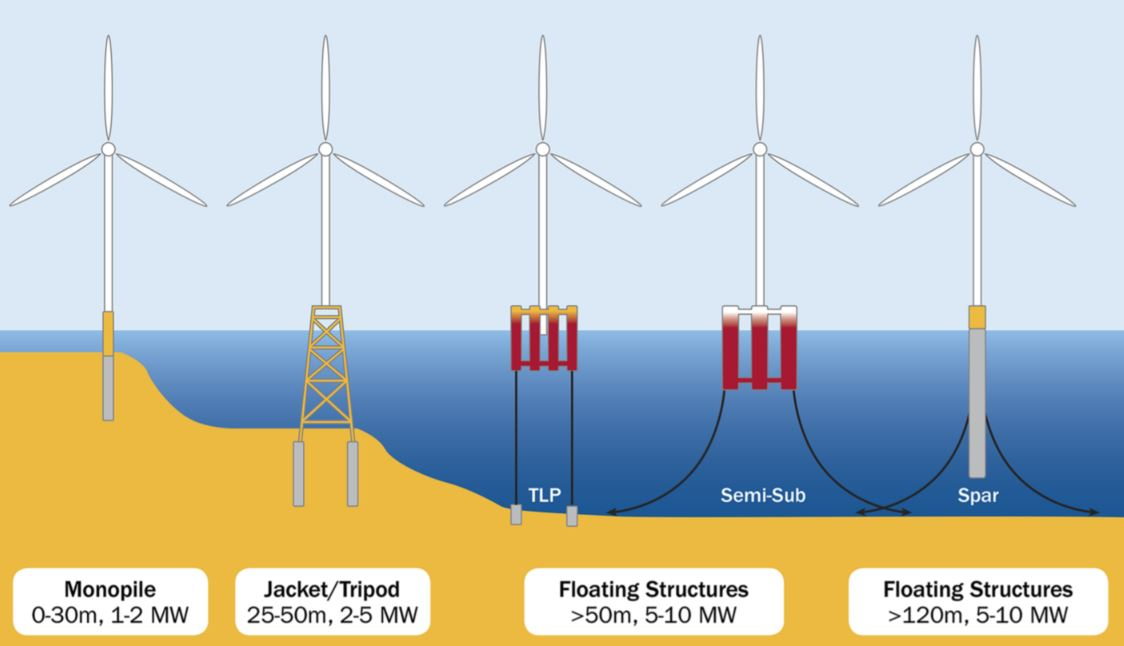
\includegraphics[scale=0.6]{figures/supstruc}
\caption[$\; \:$Different support structures]{Different support structures, \cite{Bailey2014}}
 \label{fig:supstruc}
\end{figure}

\noindent There are several pros and cons to the different designs, taken from \cite{IRENA2016}: \newline
\newline
\textbf{Tension Leg Platform (TLP)}: Very buoyant structure connected to tensioned tendons secured to the seabed by piled or suction anchors.

\begin{varwidth}[t]{.5\textwidth}
Pros :
\begin{itemize}
\item Low mass
\item Lower critical wave induced motions
\item May be assembled onshore
\end{itemize}
\end{varwidth}% <---- Don't forget this %
\hspace{4em}% <---- Don't forget this %
\begin{varwidth}[t]{.5\textwidth}
Cons :
\begin{itemize}
\item Stability issues during installation and transportation
\item May need special purpose vessel for installation
\item Higher mooring cost
\item Some uncertainty around high frequency dynamic effects
\end{itemize}
\end{varwidth}
\newline
\newline

\noindent \textbf{Semi submersible}: Submerged pontoons. Kept in position by mooring lines

\begin{varwidth}[t]{.5\textwidth}
Pros :
\begin{itemize}
\item May be assembled onshore
\item Low drought, may be transported fully equipped using tugs.
\item Lower mooring costs 
\end{itemize}
\end{varwidth}% <---- Don't forget this %
\hspace{4em}% <---- Don't forget this %
\begin{varwidth}[t]{.5\textwidth}
Cons :
\begin{itemize}
\item Higher critical wave induced motions
\item Large structures, use more material
\item Complex fabrication
\item Higher mooring cost
\end{itemize}
\end{varwidth}
\newline 

\noindent \textbf{Spar Buoy}: A cylinder with high drought with ballast below the center of gravity. kept in position with mooring lines

\begin{varwidth}[t]{.5\textwidth}
Pros :
\begin{itemize}
\item Lower critical wave induced motions
\item Simple design.
\item Lower mooring costs 
\end{itemize}
\end{varwidth}% <---- Don't forget this %
\hspace{4em}% <---- Don't forget this %
\begin{varwidth}[t]{.5\textwidth}
Cons :
\begin{itemize}
\item Installation requires heavy lift vessel
\item Needs high water depths. 
\end{itemize}
\end{varwidth}


\section{Subsea Power Cables}
 The cabling system is a crucial component for the offshore wind energy installation. Electrical power cables are used in offshore wind technology to provide energy from the wind turbine to shore or the other way around. It can also be used to provide power to other installations at sea \cite{Nasution2013}.  \cite{srinil2016} describes that the cable industry has experienced a significant increase in the demand for subsea power cables. As technology pushes installations further from shore, and into deeper waters with tough conditions, technical advances are needed for the power cables as well. For safe and efficient transfer of electricity, cable designs must be optimized according to the location of the system, infrastructure, and technical properties. " [...]to significantly increase offshore wind capacity, the inter-array and export cabling systems have been identified by the offshore wind industry as one of the key areas where related cost savings should be considered."  \cite{srinil2016}. The design of offshore power cables has several technical and economic challenges, where the distance from shore is an important parameter. According to \cite{Lynn2011}, it is most economical to use 3-phase high-voltage AC transmission for distance up to 50 km.\newline
 \newline
 \cite{Thies2012} states that there is substantial experience with marine power cables due to the large oil and gas industry. However, there is little knowledge about the loading regimes for floating marine energy converters because the technology is still relatively new and is lacking experience. 
 \newline
 \newline
 There are several different cables in use to transport the generated electricity from the wind turbine to shore, or an offshore installation, illustrated in Figure \ref{fig:diffcable} This project focuses on the dynamic part of an inter-array cable between the floating structure and the seabed. 
 
 \begin{figure}[H]
\centering
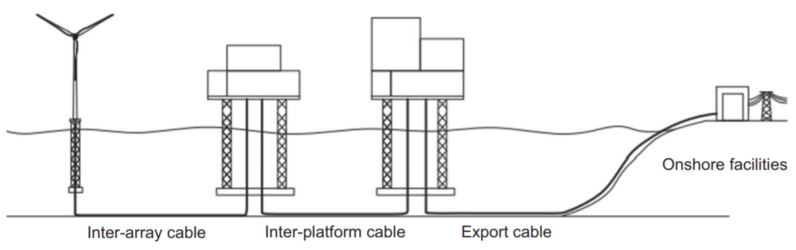
\includegraphics[scale=0.8]{figures/diffcable}
\caption[$\; \:$Different subsea power cable]{Different subsea power cables for different use. Adapted from   \cite{srinil2016} }
 \label{fig:diffcable}
\end{figure}

\noindent As can be seen in Figure \ref{fig:diffcable}, an inter-array cable link up several wind turbines to an offshore substation where the electricity is collected and transformed before it is sent to shore. \cite{srinil2016} describes that the inter-array cable is usually quite short, usually less than 1500m, depending on the size of the installation, and the spacing requirements between turbines. Inter-array cables are usually three-core copper conductors, armored with steel wires with insulation around the conductors. 33kV is usually the standard for offshore cables; however, 66kV is under development. \newline
\newline
  
  \subsection{Dynamic Power Cables}
According to \cite{Thies2012}, power cables can be used in static applications, where it is connected to a fixed structure, or dynamic application where it has to withstand significant cyclic loading. \cite{srinil2016} stats that "For offshore floating wind turbines, attention must be paid to the development, design, and optimization of a robust dynamic power cable." The combination of the different loads from waves, wind, currents, and more are complex and need to be assessed through a coupled model and experimental tests. \\\\
\subsection{General Design of Subsea Power Cable}
There are several different designs of subsea power cables. According to \cite{Beckman}, each cabling system is specially designed for its purpose, making repairs and maintenance challenging. \cite{Thies2012} describes some of the most common features for a standard subsea power cable presented in Figure \ref{fig:pcable}: 

\begin{enumerate}[label=\Alph*]
\item Conductor core: Carry the electrical current, and consists of wires made of copper or aluminum. 
\item Electrical insulation: Insulating the conductors. Possible materials are oil-impregnated paper, cross-linked polyethylene, or ethylene propylene rubber.
\item Sheath: Acts as a water barrier, and to protect the cable against fault currents. 
\item Armature: Metallic armature usually two layers of galvanized steel wires. Gives mechanical strength and protects against impact
\item Protective sheath: Outer layer of cable gives abrasion strength, and is made out of polypropylene
\end{enumerate}

\noindent Optical cables may be included in the cross section for some applications. Cables need to be optimized for their use, and standardized cables are rather rare. 


\begin{figure}[H]
\centering
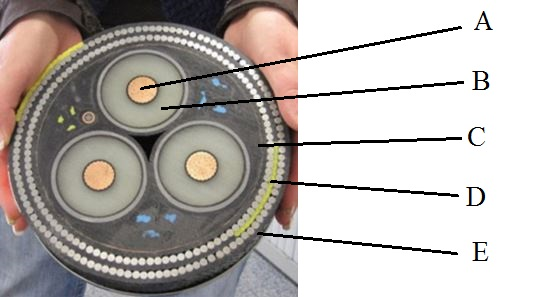
\includegraphics[scale=0.8]{figures/pcable}
\caption[$\; \:$Main components of a typical subsea power cable]{Main components of a typical subsea power cable. Adapted from \cite{Boltinha2016} }
 \label{fig:pcable}
\end{figure}

\noindent As mentioned in Section 1.3.2, the W-configuration is not the only configuration that has been used for inter-array cables in recent years, and other configurations are being explored. Figure \ref{fig:config} shows some of the most common riser configurations for floating offshore structures. 

\begin{figure}[H]
\centering
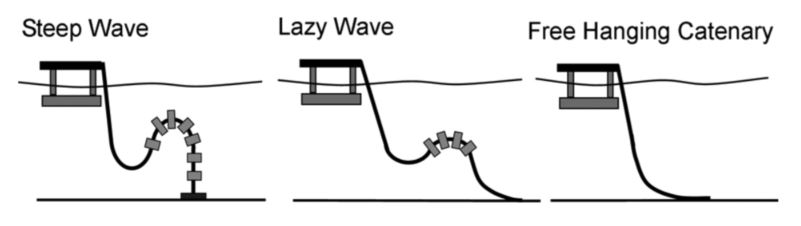
\includegraphics[scale=0.8]{figures/config}
\caption[$\; \:$Different configurations of flexible riser]{Different configurations of flexible riser, \cite{Thies2012}}
 \label{fig:config}
\end{figure}

\noindent For the 1st and 2nd configuration in Figure \ref{fig:config}, buoyancy modules need to be designed to obtain the desired shape, according to \cite{srinil2016}. These are usually made of synthetic foam. They are positioned on the central part of the flexible riser/power cable and held in place with internal clamps. Using the steep wave or the lazy wave configuration usually minimizes the dynamic response of the cable,  decoupling the floating structure motion from the cable touch down point on the seabed. The configuration is highly dependent on the buoyancy elements, so these should not be changed over the lifetime of the flexible cable. Figure \ref{fig:bend} shows how buoyancy elements change the configuration of the flexible riser in terms of hang-off, arch bend, and touch down. "Depending on the hang-off angle, water depth, platform offset, footprint and soil stiffness, areas of local maximum static tensions typically occur at the hang-off point and
the two ends [...] of the distributed buoyancy portion[...]" \cite{srinil2016}. The local maximum bending moments happen where the largest curvature occurs.

\begin{figure}[H]
\centering
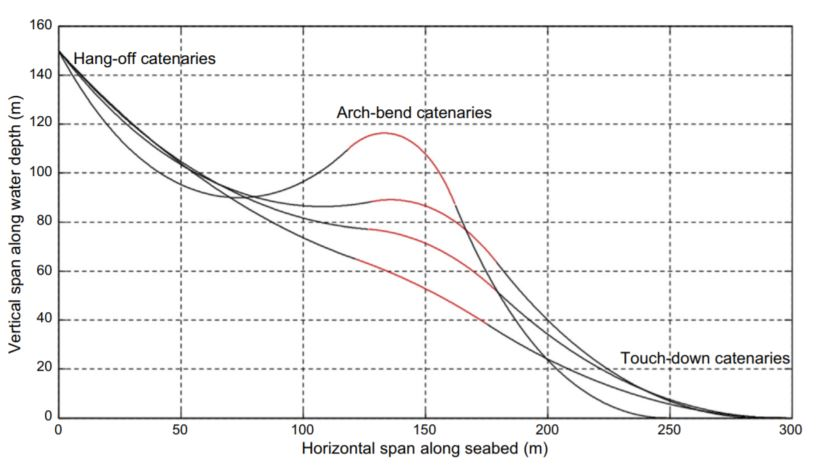
\includegraphics[scale=0.6]{figures/bend}
\caption[$\; \:$Effect of buoyancy distribution]{"Effect of buoyancy distribution (red line) change on the configuration of dynamic
cable", \cite{srinil2016}}
 \label{fig:bend}
\end{figure}
\subsection{Bend Stiffener}
The information in the following paragraph is taken from \cite{Worzyk}. \\\\
A dynamic power cable is susceptible to fatigue or over bend when there is an abrupt change in bending stiffness. This can be the case several places including at the cable hang off. An over-bend of the cable may lead to severe fatigue damage. To reduce the effect of changing bending stiffness, a bend stiffener may be incorporated in the cable structure. A bend stiffener is a conical structure attached around the cable at the cable hang off. Its conical shape makes the increase of bending stiffness more gradual, and each bend stiffener requires individual design. A poorly designed bend stiffener simply relocates the problem to the end of the bend stiffener.


\subsection{Copper Power Conductors}
  According to \cite{Worzyk}, the majority of subsea power cables include conductors made of copper. Copper is often superior to aluminum for subsea applications, as it allows for smaller cross-section, and thus requires less material for the steel armoring around it. There are several  types of conductors as can be seen in Figure \ref{fig:conductors}
  \begin{figure}[H]
\centering
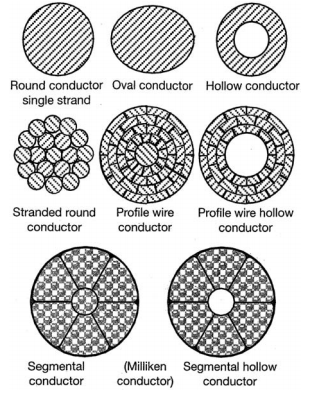
\includegraphics[scale=0.6]{figures/conductors}
\caption[$\; \:$Different types of conductors]{Different types of conductors, \cite{Worzyk} }
 \label{fig:conductors}
\end{figure}
 Stranded round cables are most prevalent for subsea application. \cite{Nasution2013} explains that the wires are arranged in layers, and the conductors may be of different sizes with a different number of layers. According to \cite{Worzyk} the wires are compressed in stranding machines in layers, or at the end of the stranding. The compression reduces the space between the circular wires, and a compressed copper cable may have a fill factor up to 0.92. 
  \\\\
 \cite{Nasution2013} elaborates: The helical nature of the wires in each layer leads to different contact between the wires. Contact between wires of the same layer is called inline contact, while contact between wires of different layers is called trellis contact. The inline and trellis contact between the wires can be seen in Figure \ref{fig:cross}, where the red arrows indicate inline contact, and the black arrows indicate trellis contact. 
  \begin{figure}[H]
\centering
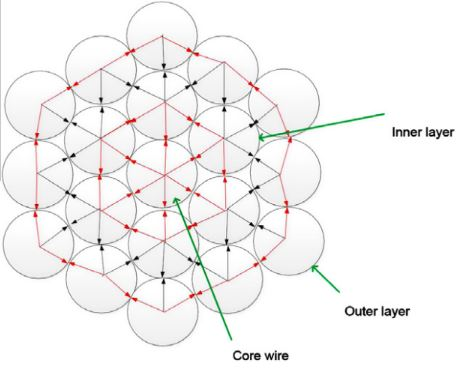
\includegraphics[scale=0.9]{figures/cross}
\caption[$\; \:$Inline and trellis contact between wires]{Inline and trellis contact between wires, \cite{Nasution2013} }
 \label{fig:cross}
\end{figure}

\noindent The loads on the cables are transferred to the individual wires in the copper conductor. The dynamic and mean tension, are transferred as tension and shear force, and the dynamic bending moment gives local bending and axial friction forces. This can be seen in Figure \ref{fig:cable}, where:
\begin{itemize}
    \item $\overline T$ is the mean tension
    \item $\Delta T$ is the dynamic tension
    \item $\overline M_T$ is the mean bending moment
    \item $\Delta M_T$ is the dynamic bending moment
    \item $\Delta \beta$ is the dynamic curvature
    \item $\overline F_X$ is the mean axial force
    \item $\Delta F_X$ is the dynamic axial force
    \item $\overline T$ is the mean tension
    \item $\Delta M_X$ is the dynamic torque moment about helix tangential x-direction
    \item $\Delta M_y$ is the dynamic bending moment about helix bi-normal y-direction
    \item $\Delta M_z$ is the dynamic bending moment about surface normal z-direction
\end{itemize}


\begin{figure}[H]
\centering
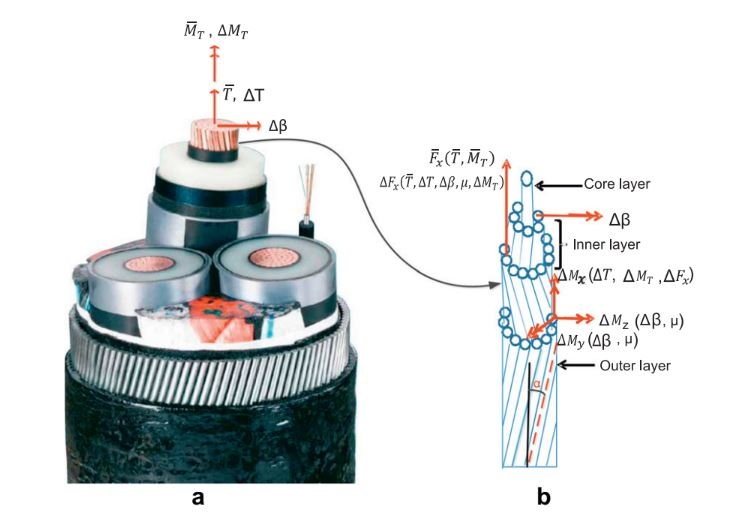
\includegraphics[scale=0.8]{figures/cable}
\caption[$\; \:$Forces on cable]{Forces on cable,  \cite{Nasution2013} }
 \label{fig:cable}
\end{figure}

\subsection{Alternating current (AC) Voltage}
Electrical power can be supplied either by direct current, (DC) or alternating current, (AC). DC only flows in one direction, while for AC, the direction of the current changes direction several times over a time unit as a sine function, \cite{Dale2000}. Figure \ref{fig:acdc} compares the waveform for DC current and AC current.


\begin{figure}[H]
\subfloat[Waveform for DC voltage \label{fig:dc}]
  {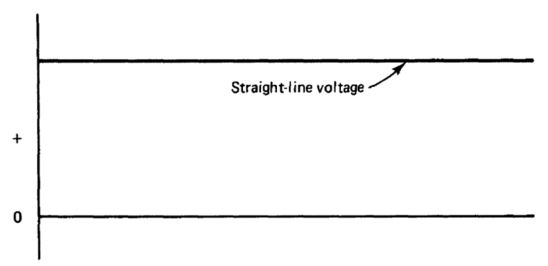
\includegraphics[width=.45\linewidth]{figures/dc}}\hfill
\subfloat[Waveform for AC voltage \label{fig:ac}]
  {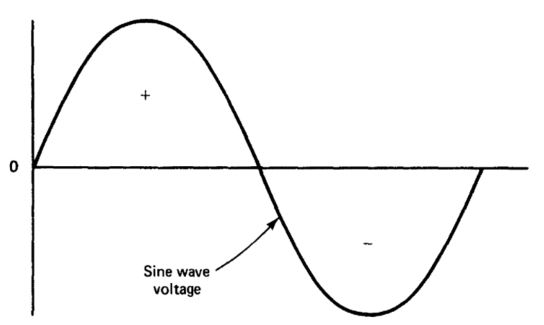
\includegraphics[width=.45\linewidth]{figures/ac}}\hfill
\caption[$\; \:$Comparison of DC voltage and AC voltage]{Comparison of DC voltage and AC voltage, \cite{Dale2000}}
\label{fig:acdc}
\end{figure}

\noindent A three-phase system is made up of three coils rotating in a magnetic field with a phase difference of 120$^{\circ}$, \cite{Dale2000}. The three-phase system and its alternating voltage can be seen in Figure \ref{fig:volt}. According to \cite{Beckman}, an AC cable requires one conductor for each phase. The three conductors may be placed in the same cable or within three individual cables. AC demands a thicker cable cross-section than DC, but smaller transformers.

\begin{figure}[H]
\subfloat[Single phase AC voltage \label{fig:single}]
  {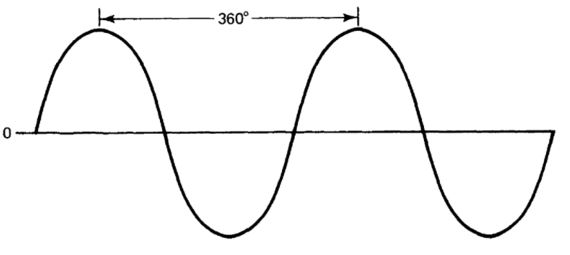
\includegraphics[width=.45\linewidth]{figures/single}}\hfill
\subfloat[Three phase Ac voltage \label{fig:3phase.JPG}]
  {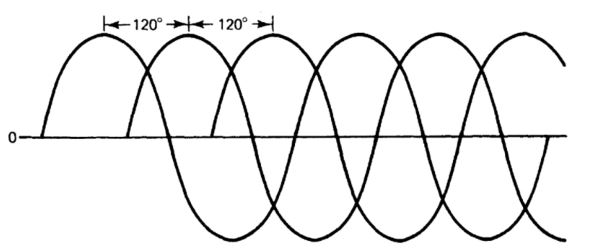
\includegraphics[width=.45\linewidth]{figures/3phase}}\hfill
\caption[$\; \:$Comparison of single phase and three phase AC voltage]{Comparison of single phase and three phase AC voltage, \cite{Dale2000}}
\label{fig:volt}
\end{figure}

\noindent There are several advantages with three-phase AC systems over 1 phase AC systems in terms of price, material use, robustness,"[...] and accounts for the vast majority of the world's industrial machines", \cite{1995Tac}.
 


